\documentclass[]{article}
\usepackage{hyperref}
\usepackage{multicol}
\usepackage{graphicx}
\usepackage{xcolor}
\usepackage{listings}
\usepackage{xparse}

\setlength{\columnsep}{0.7cm}
\usepackage[backend=bibtex]{biblatex}
\usepackage[a4paper, total={6in, 8in}]{geometry}
%opening
\title{Report Biomarkers}
\author{Benedetta Corso, Letizia Rossato, Dalila Dattoli}
\addbibresource{bibliog.bib}

\NewDocumentCommand{\codeword}{v}{%
	\texttt{\textcolor{blue}{#1}}%
}

\lstset{language=C,keywordstyle={\bfseries \color{blue}}}

\begin{document}

\maketitle

\begin{abstract}
This study, which focuses on Parkinson's disease, aims to investigate the significance of left-right lateralization based on dopamine values using DAT-SPECT imaging data and their correlation with clinical symptoms in Parkinson’s disease patient (PD) and healthy controls (HC). DAT-SPECT (Dopamine Transporter Single Photon Emission Computed Tomography) is an imaging technique primarily used to visualize and measure the density of dopamine transporters in the brain.  Indeed, this technique is particularly useful in the diagnosis and evaluation of neurodegenerative diseases, such as Parkinson's disease and other forms of parkinsonism. The dataset, used to perform the analysis, consists of variables relating to demographic data, DAT-SPECT scores and finally the Neuropsychological (NP) tests which are a combination of clinical, neurological, and imaging test since there is no specific test for the diagnosis of Parkinson’s disease. In order to investigate whether the lateralization is related to symptoms, a linear regression approach was used. This analysis verified that the lateralization is highly related to symptoms in PD patients.
The lateralization of dopamine function could be useful in the future as a possible biomarker of PD symptoms severity.

LAT COEFFICIENT OR INDEX CAMBIARE DAPPERTUTTO
CONTROLLARE SINGOLARE O PLURALE DI DATA

\textcolor{red}{ADD RESULTS}
\newline

\end{abstract}

\begin{multicols}{2}
\section{Introduction}
Parkinson's disease is a chronic neurodegenerative disorder of the central nervous system primarily affecting motor control. It is characterized by the progressive loss of nerve cells in the brain region called the substantia nigra, which is responsible for producing a neurotransmitter called dopamine. Dopamine deficiency leads to motor symptoms such as tremors, muscle rigidity, bradykinesia (slowness of movement), and postural instability. In addition to motor symptoms, Parkinson's disease can cause a wide range of non-motor symptoms including sleep problems, depression, anxiety, fatigue, and cognitive difficulties. While the exact cause of Parkinson's disease is not fully understood, it is believed to result from a combination of genetic and environmental factors \cite{beitz_parkinsons_2014}. Currently, there is no cure for Parkinson's disease, but there are treatments available to manage symptoms and improve the patients’ quality of life.  However, studies conducted in recent years have shown that the lateralization of brain dopamine in Parkinson's disease (PD) is a significant and distinctive aspect of the pathology. In particular, during its development, the degeneration of dopaminergic neurons in the substantia nigra is not uniform. Generally, one side of the brain is more affected than the other, leading to marked asymmetry. This marked asymmetry is visible not only in motor symptoms, such as more pronounced tremors on one side of the body and greater use of one hand over the other, but it can also be evident in non-motor disturbances, including cognitive issues for example in the sleep behavior and or sense of smell \cite{riederer_lateralisation_2018}. 
\newline
In previous studies, the connection between dopamine lateralization and symptoms has already been examined. For example, in \cite{pirker_correlation_2003}, it resulted that the motor symptoms on the less affected side were more correlated to striatal DAT binding.
\newline
Therefore, the aim of this study is to further investigate this idea, analyzing a dataset containing information about patients' motor and cognitive symptoms and also their lateralization data obtained from DAT-SPECT scans. The dopamine degeneration is explored in three different Regions of Interests (ROIs) in the brain, divided in right and left: Caudate, Putamen and Putamen Anterior. This analysis aims to investigate the relationship (if present) between the lateralization of dopamine function in these brain areas and the symptoms showed by Parkinson's patients, and relationship (if present) between the lateralization of dopamine function in these brain areas and possible covariates shown by healthy controls. To do so, the group checked also if there was a difference in lateralization between HC and PD. 
\newline
Agreeing with what found in \cite{pirker_correlation_2003}, the group expected to find a strong relation between the dopamine lateralization and the motor symptoms. The lateralization was expected to be significantly different between the two groups of HC and PD. Also the lateralization in different ROIs was expected to be related: a high lateralization in the Caudate was expected if both Putamen and Putamen Anterior were highly lateralized. 

\section{Material and Methods}

\subsection{Dataset description}
The dataset used in this study was composed of 1556 subjects, of which 256 healthy controls and 1300 PD patients with different levels of symptoms' severity. Not all the variables given were interesting for the study. For example, all the data regarding the MRI acquisitions were discarded, because the analysis focused on the data from the DAT-SPECT scans, which were Striatal Binding Ratios (SBR) of the three ROIs (right and left sides), whether the scan was completed and its quality based on visual interpretation, as well as information regardind the date of the scan and the injection. 
\newline
The dataset included a part of demographics data, like age, ethnicity, gender, family members affected by PD, height, weight and dominant hand.
A total of 967 and 589 patients were males and females, respectively. The average age in the baseline was 62.69 ± 10.11 years (range [29.3–86.5]). 

There was then the data regarding the neuropsychological assessments of the patients using the Movement Disorder Society (MDS)-sponsored revision of the Unified Parkinson's Disease Rating Scale (MDS-UPDRS). The test is divided in 4 parts, concerning different classes of motor and cognitive symptoms, as specified in the PPMI Program Protocols (THE PARKINSON'S PROGRESSION...). Each answer could range from 0 (normal) to 4 (severe), and for each part there was a summing-up variable, that contained the sum of all the scores of that section. These variables were called NP1PTOT, NP1RTOT, NP2TOT, NP3TOT, NP4TOT. Some motor symptoms, especially in the third part, were divided in right and left, for example, the severity of tremor of the right or left upper limb. This was useful to investigate the different relation with the dopamine function lateralization.
\newline

Più aggiungere forse grafici con distribuzioni variabili iniziali, tipo grafici lateralizzazione

\subsection{Cleaning e preprocessing}

The first step was dividing the dataset in patients (PD, SWEDD, Prodromal) and HC.

In the preprocessing of the data, the patterns of missing values were analyzed, to determine the best course of action, through the VIM package in R.

In the HC, as shown in figure \ref{fig:missing_patterns_HC}, GENETICS and FAMILIARITY are mostly empty fields, due to the nature of these variables: for healthy subjects, the chance of having relatives with a PD diagnosis and of having genetics history related to PD are low. On the opposite, for PD patients (figure \ref{fig:missing_patterns_PD}), GENETICS is empty at the TOT \%, while FAMILIRITY has the TOT \% of NaNs. The reason for this missingness, is probably that patients didn't know if their relatives had history of Parkinson's, or they didn't take the genetics test. 

In the complete dataset, NP4TOT is missing at the 73.9\%; nearly all the HC didn't take the fourth part of the test, and also the participation of the PD was really low. This suggests that the fourth part of the test was taken by a few subjects. For this reason, the NP4 variables were not taken into account in the statistical analysis.

For all the test-related variables (NP1PTOT, NP1RTOT, NP2TOT, NP3TOT), both in HC and PD, if a subject is missing a value for one test, also the other tests' results are missing. The pattern of missing data is considered to be MAR (Missingness At Random). For the statistical analysis, all the subjects that were missing at least one test result weren't considered.  

For ETHNICITY, SEX, and HAND (dominant hand of the subject), there aren't missing valules in the whole dataset. In the ENROLL\_AGE variable, the missing values were calculated using the DAT-SCAN date and the birth date of the subject.

Regarding HEIGHT and WEIGHT, the pattern of missing data is MAR, with a total of TOT \% of NaNs. 

The variable PRIM\_DIAG described the primary diagnosis; the group found some subjects with the value of 97, that wasn't explained by the data dictionary, therefore it was removed both from the HC and from the PD. 

In figures \ref{fig:HC_missing_values} and \ref{fig:PD_missing_values}, all the combinations of missing values of the dataset have been represented, using the VIM package in R.


\end{multicols}

\begin{figure}[h]

	\centering
	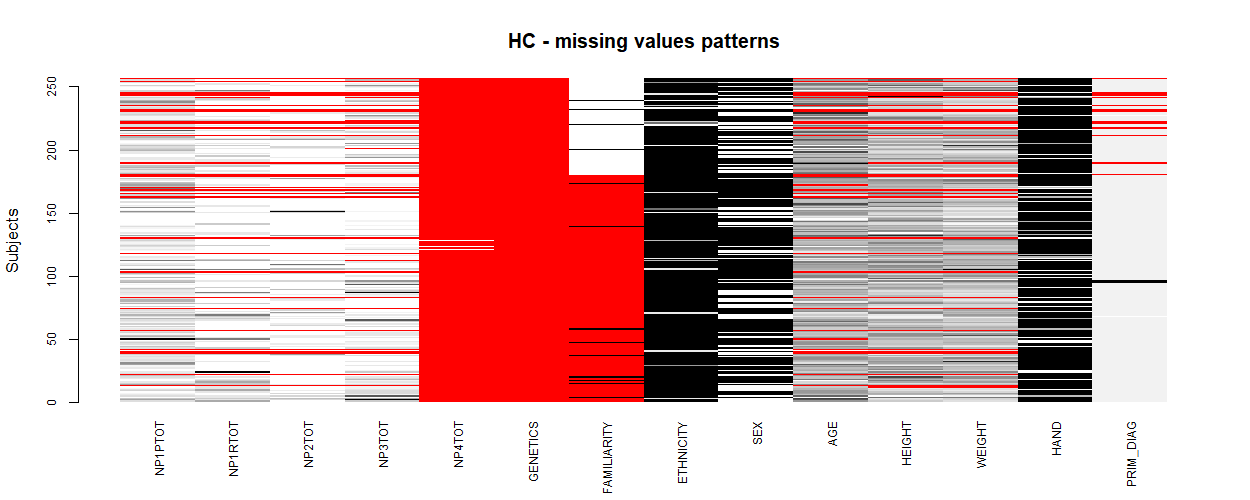
\includegraphics[width=4in]{../missing_patterns_HC}
	\caption{Pattern of missing values in HC}
	\label{fig:missing_patterns_HC}

	\centering
	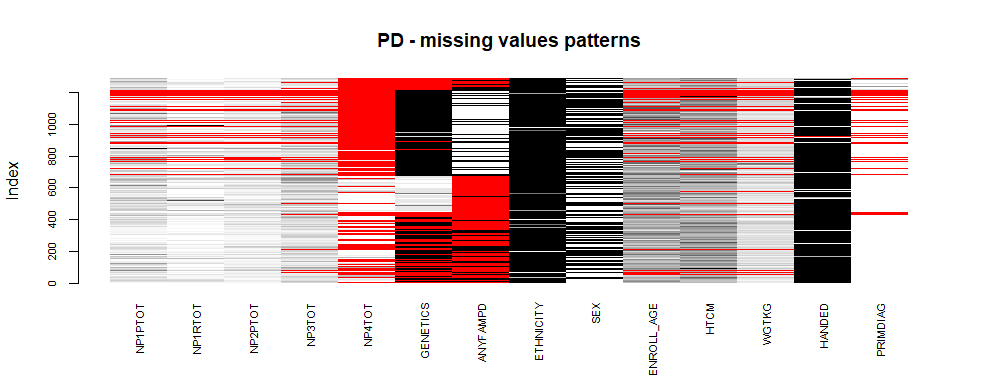
\includegraphics[width=4in]{../missing_patterns_PD}
	\caption{Pattern of missing values in PD}
	\label{fig:missing_patterns_PD}
	
\end{figure} 
\begin{figure}[h]
	\centering
	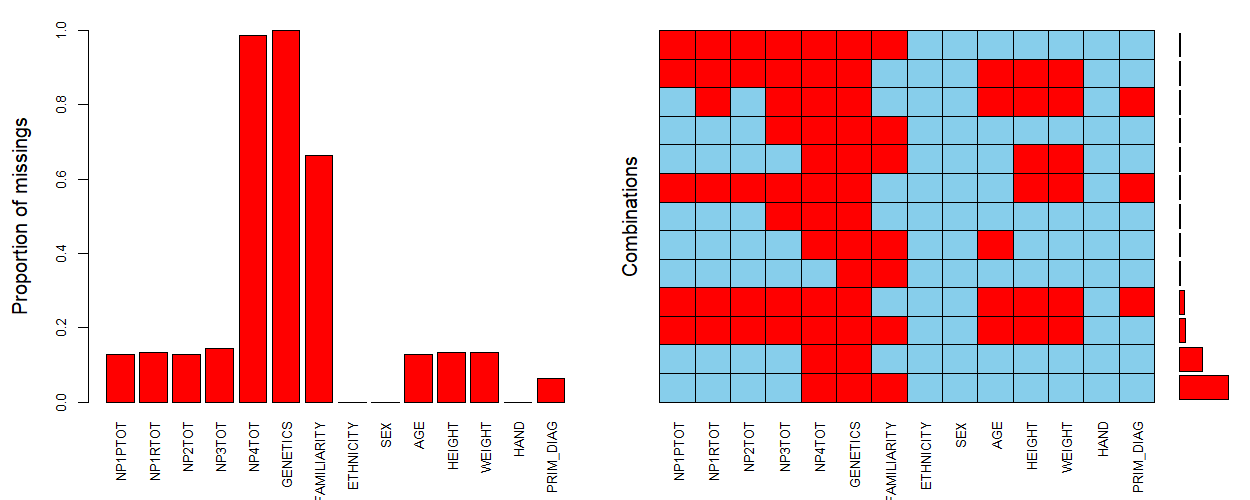
\includegraphics[width=2.4in]{../missing_values_HC}
	\caption{Missing values in HC}
	\label{fig:HC_missing_values}
	
	\centering
	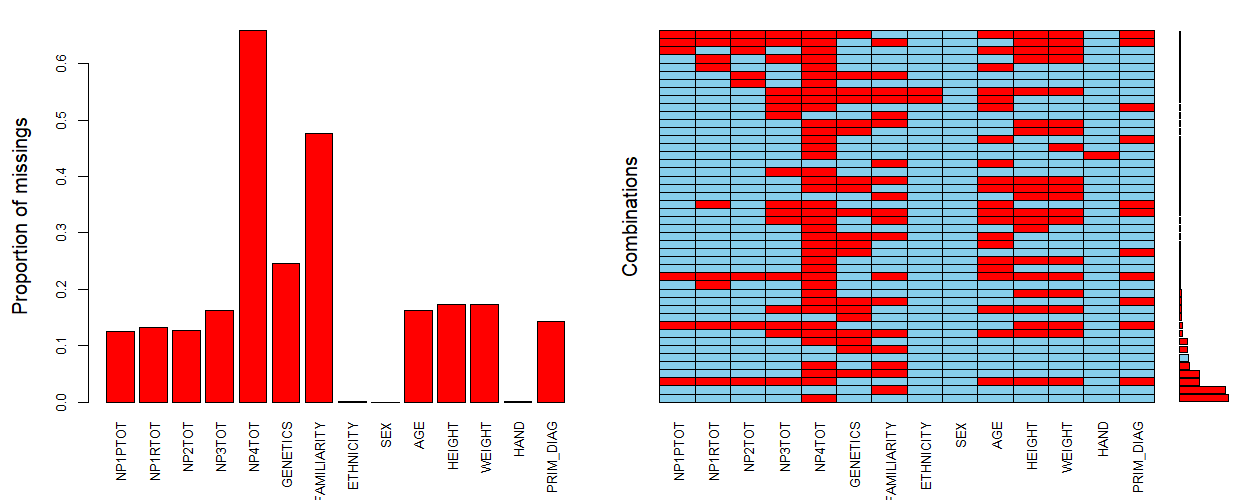
\includegraphics[width=2.4in]{../missing_values_PD}
	\caption{Missing values in PD}
	\label{fig:PD_missing_values}

\end{figure} 


\begin{multicols}{2}

Another reason of exclusion from the analysis, was having an incomplete DAT-SCAN, a scan with poor quality, or, just for HC, a MoCA (Montreal Cognitive Assessment - stored in the variable MCATOT), score lower than 26. This test assesses the cognitive impairment, and, under 26, the subjects couldn't be considered healthy. 

The preprocessing step ended with the removal of some outliers from ENROLL\_AGE, HEIGHT and WEIGHT. (DA CONTROLLARE)

Concerning the demographics data, the two datasets were compared, to see if they had the same distributions. Through the Anova test, the average values of age, height and weight were found identical for the two groups. The proportion of male and female was comparable: in the whole dataset, the proportion of females was 37,85\%, while in PD was 38,5\% and in HC 34,37\%. 

The distribution of ETHNICITY was also found similar between the two groups, while FAMILIARITY and HAND were significant different in the two populations when analyzed through a Wilcoxon test. The differences in FAMILIARITY can be explained by the connection between PD patients and the genetic components in the disease: for a PD patient, it's more likely to have some relatives affected by PD, than for an healthy subject. 


\subsection{Feature extraction}

In order to perform the statistical analysis to answer the study questions, the relevant features were extracted.
The analysis was based on the DAT-SPECT data, for the three ROIs, the demographic data and the symptoms tests results. Therefore, the MRI data were discarded.

\subsection{Lateralization indexes}

From the lateralization data, the group used a DAT binding asymmetry index found in \cite{kaasinen_ipsilateral_2016}: (right - left SBR)/(right + left SBR). The lateralization was considered relevant when the asymmetry index was higher than 20\%.
This threshold level was adopted from a previous study \cite{fiorenzato_asymmetric_2021}. In this way, the group identified, for the Caudate,  28 PD patients with a right lateralization and 29 with a left lateralization. For the Putamen, 203 PD had a right lateralization, 2 HC and 150 PD with a left lateralization. For the Putamen Anterior, 113 PD patients were found lateralized on the right side, while 64 on the left. The remaining subjects were not lateralized.

\subsection{Covariates analysis}

Analyzing HC, the possible covariates were sex, dominant hand, ethnicity, age, height, weight.

Regarding the discrete variables, it was possible to analyze only SEX, because the others didn't divide the subjects in groups with a comparable number of data. 
The lateralization indexes were, for each region, divided in males and females. Through a Lillie test, both groups were found not gaussian. Therefore, they were compared with a Wilcoxon test, finding that for all the three regions, males and females had different medians of lateralization indexes.
Consequently, SEX was considered as a covariate for the study, and the statistical analysis on PD patients was performed both on the whole group and on the two sub-groups of males and females.

Through the Pearson pairwise correlation, the group analyzed the correlation coefficients of the continue variables, such as ENROLL\_AGE, WGTKG (weight - kg), HGTCM (height - cm), with the lateralization indexes (figures \ref{fig:cov_mat_hc}). For the statistical analysis, were kept only the significant ones, with p-value $<$ 0.05, and correlation coefficient higher than 0.5. This threshold was chosen in order to have at least a moderate correlation (0.4-0.59). 

\end{multicols}

\begin{figure}[h]
	\centering
	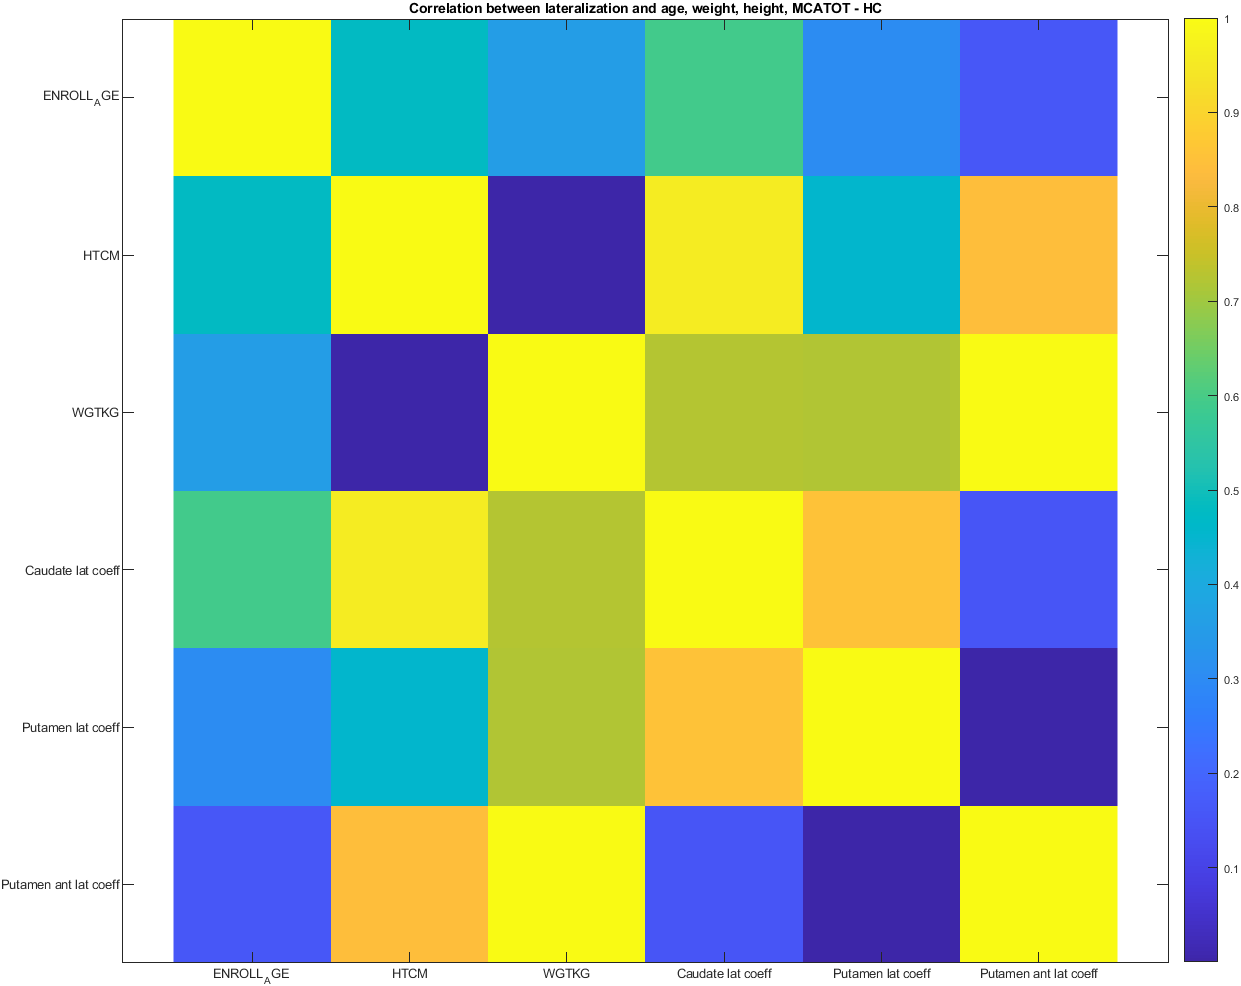
\includegraphics[width=3in]{../covariates_mat_hc}
	\caption{Correlation matrix between covariates and lateralization index - HC}
	\label{fig:cov_mat_hc}
\end{figure} 
 
\begin{multicols}{2}

In the correlation matrix of the HC in figure \ref{fig:cov_mat_hc}, it's shown that ENROLL\_AGE has a moderate correlation only with the lateralization coefficient in the Caudate region, while it has a weak correlation with the other two ROIs. HTCM is strongly correlated with Caudate's lateralization coefficient, moderately with Putamen and has a very strong correlation with Putamen Anterior. Similarly, also WGTKG has a very strong correlation with Putamen Anterior, and a strong one with Caudate and Putamen lateralization indexes.

\subsection{Statistical methods}

The group used the Pearson correlation coefficient in the covariates analysis and in the symptoms analysis.

The Anova test was used in the pre-processing section in order to compare the distributions of HC and PD continuous variables (age, height, weight).
Also, the Wilcoxon test was used during the pre-processing step, but to compare the discrete variables distributions (sex, familiarity, ethnicity).

Then the group compared HC and PD populations in terms of lateralization, using an Anova test (figures \ref{fig:anova_table} and \ref{fig:anova_plot}). The Anova test was chosen because the normality assumption wasn't met, and so the T-test couldn't be used.
Therefore, the analysis investigated the presence of a difference between the lateralization in HC with the one in PD. To perform the analysis, the lateralization was taken in absolute value. The choice of using the absolute value came from the interest on the amount of lateralization, not its direction.

\subsubsection{Linear regression}

Using the covariates variables (found for HC through the correlation matrix) and the symptoms data, the group performed a linear fit with the lateralization indexes of PD patients, to check the presence of a linear relation between them. 
This was implemented through the MATLAB function \codeword{fitlm} (the lateralization was not take in absolute value, in order to have a relation with its direction).
As parameter, the adjusted $R^2$ was used to get the true value of the fit.

\section{Results}

The covariates extracted for each ROI are shown in Table \ref{tbl:cov_hc}.

\end{multicols}

\begin{table}[h]
	\centering
	\begin{tabular}{|c|c|c|}
		\hline
		\textbf{ROIs}             & \textbf{Covariates} & \textbf{Correlation coefficient} \\ \hline
		\textbf{Caudate}          & ENROLL\_AGE         & 0.593                            \\ \hline
		\textbf{}                 & HTCM                & 0.958                            \\ \hline
		\textbf{}                 & WGTKG               & 0.723                            \\ \hline
		\textbf{Putamen}          & WGTKG               & 0.722                            \\ \hline
		\textbf{Putamen Anterior} & HTCM                & 0.840                            \\ \hline
		\textbf{}                 & WGTKG               & 0.997                            \\ \hline
	\end{tabular}
	\caption{Covariates correlation coefficients - HC}
	\label{tbl:cov_hc}
\end{table}

\begin{multicols}{2}

The results of the Anova test to compare the lateralization indexes of PD and HC are shown in Figures \ref{fig:anova_table} and \ref{fig:anova_plot}.
As hypothesized at the start of the study, the analysis confirmed that there was a significant difference (p-value $<$ 0.01) in the lateralization of HC and PD in all the ROIs.

\end{multicols}

\begin{figure}[h]
\centering
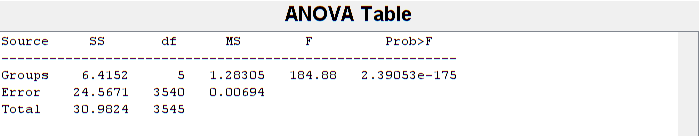
\includegraphics[width=3in]{../anova_table_lat_hc_pd}
\caption{Anova test results, comparing lateralization indexes in PD and HC}
\label{fig:anova_table}
\end{figure} 

\begin{figure}[h]
\centering
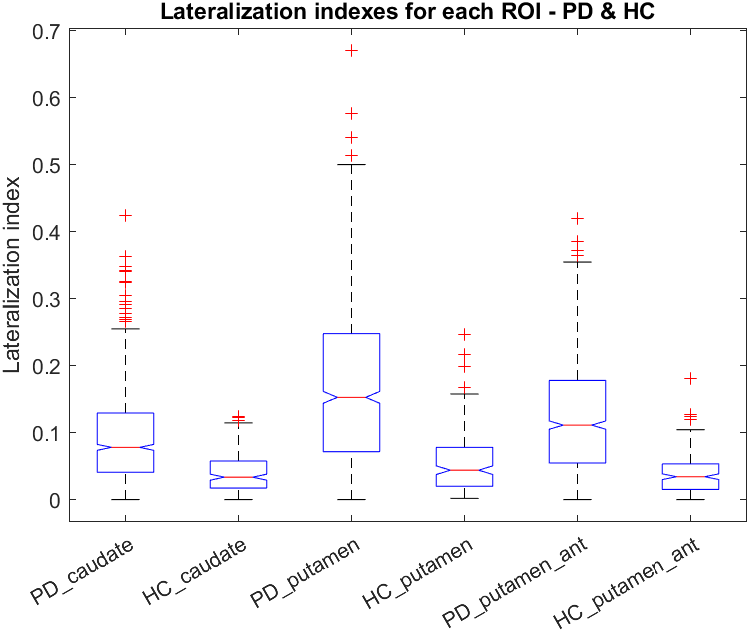
\includegraphics[width=3in]{../anova_plot_lat_hc_pd}
\caption{Anova test boxplots, comparing lateralization indexes in PD and HC}
\label{fig:anova_plot}
\end{figure} 

\begin{multicols}{2}

\subsection{Symptoms correlation matrix}

To answer the first research question, which was to investigate the relationship between dopamine lateralization function and symptoms, the group extracted the significant symptoms from a correlation matrix (Figure \ref{fig:corr_symp_pd}) obtained with the Pearson correlation as done for the covariates, with a threshold of 0.5 for the correlation coefficients. 

\end{multicols}

\begin{figure}[h]
	\centering
	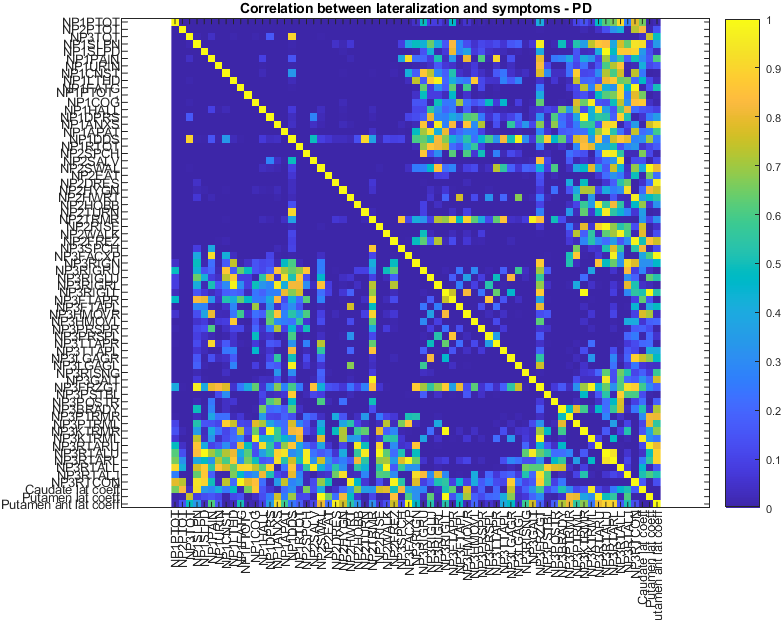
\includegraphics[width=3in]{../corr_mat_symptoms_pd}
	\caption{Correlation matrix between Lateralization indexes and symptoms - PD}
	\label{fig:corr_symp_pd}
\end{figure} 

\begin{multicols}{2}

These symptoms were used, together with the covariates found from HC, to perform a linear fit with the lateralization indexes in PD, in order to find the relationship between dopamine lateralization function and symptoms. The graphs of the fit are shown in Figure \ref{fig:lin_fit_pd}. The graphs contain on the x-axis the covariates, while on the y-axis the lateralization indexes. Each figure shows the fit for the three different ROIs, Caudate, Putamen and Putamen Anterior. 
The numerical results of these linear fits are shown in the Table \ref{tbl:R_squared_fit_pd}, where $R^2$ (adjusted) was chosen because . The p-values were all under 0.01 and therefore they aren't shown in Table \ref{tbl:R_squared_fit_pd}.

\end{multicols}

\begin{figure}[h]
	\centering
	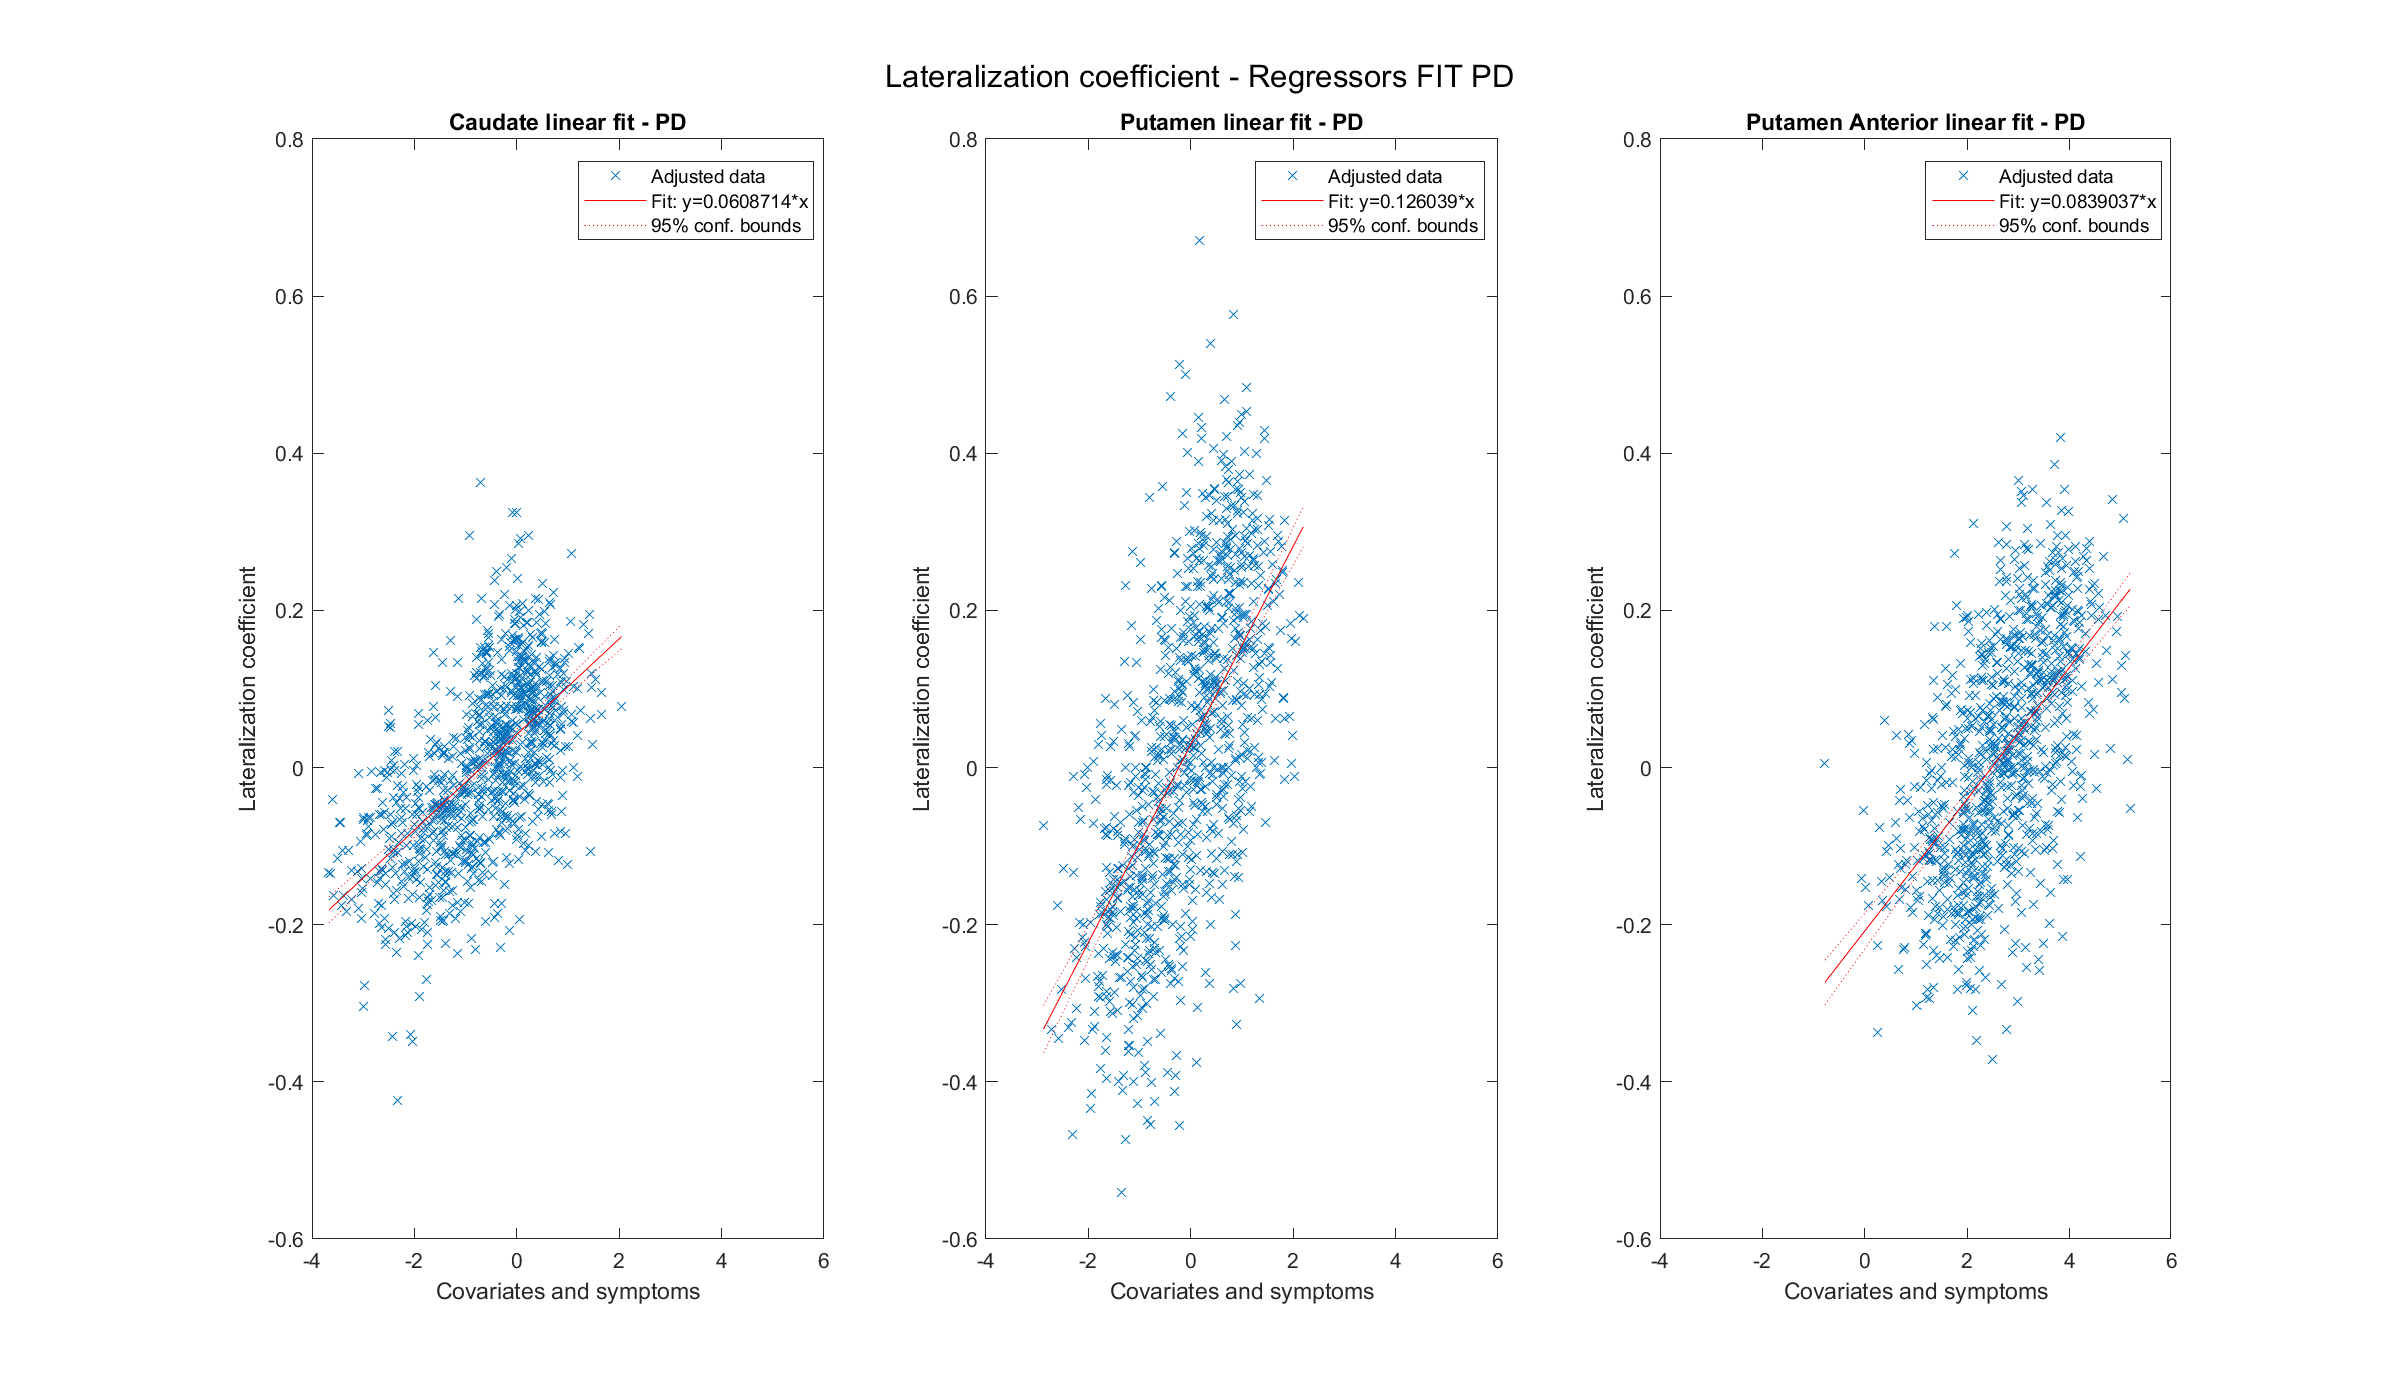
\includegraphics[width=3in]{../fit_covariates_pd}
	\caption{Linear fit - PD}
	\label{fig:lin_fit_pd}
\end{figure} 

\begin{table}[h]
	\centering
	\begin{tabular}{|c|c|}
		\hline
		\textbf{ROIs}             & \textbf{adjusted $R^2$} \\ \hline
		\textbf{Caudate}          & 0.3287                  \\ \hline
		\textbf{Putamen}          & 0.3634                  \\ \hline
		\textbf{Putamen Anterior} & 0.3014                  \\ \hline
	\end{tabular}
	\caption{Adjusted $R^2$ values of the linear fit between lateralization and symptoms}
	\label{tbl:R_squared_fit_pd}
\end{table}

\begin{multicols}{2}

FIT SENZA E CON DIVISIONE MASCHI FEMM







The second research question was whether a relationship between dopamine lateralization function and possible covariates shown by healthy controls was present. To answer this question, the following results were found. 





- A clear and concise description of the statistical results 
providing answers to the research questions
\newline
- A sensitivity analysis of the results to covariates, group matching and data quality (e.g. missing data, data miss balance)

\section{Discussion}

As shown in figures \ref{fig:lin_fit_hc} and \ref{fig:lin_fit_pd}, and from the values of $R^2$ and p-value, the group understood that the linear fit wasn't appropriate to describe the lateralization of HC, because there wasn't any significant lateralization, nor any symptoms. The image of the fit is used to show that the results are as expected. 
On the other hand, for PD patients, the values of $R^2$ and p-value are highly significant, showing that the lateralization is related to the symptoms, as hypothesized. 


HC differenza significativa con PD grazie all'indice <20 


- Direct answers to the research questions
\newline
- An overview of the limitations of the study
\newline
- A list of possible suggestions to improve the study in case 
someone will repeat it in future

\end{multicols}

\printbibliography
\end{document}
